\documentclass[11pt,a4paper]{article}

\usepackage{kotex}
\usepackage{amsmath,amssymb,mathtools,bm}
\usepackage{booktabs,tabularx,longtable,array}
\usepackage{graphicx}
\usepackage{caption}
\usepackage{subcaption}
\usepackage{geometry}
\usepackage{enumitem}
\usepackage{xcolor}
\usepackage{hyperref}
\usepackage{listings}
\usepackage{float}

\geometry{margin=25mm}
\graphicspath{{report_figures/}}
\hypersetup{
  colorlinks=true,
  linkcolor=blue!60!black,
  citecolor=blue!60!black,
  urlcolor=blue!60!black
}
\setlist[itemize]{leftmargin=2em}
\setlist[enumerate]{leftmargin=2em}
\lstset{
  basicstyle=\ttfamily\small,
  breaklines=true,
  frame=single,
  columns=fullflexible
}
\sloppy

\newcommand{\E}{\mathcal{E}}
\newcommand{\N}{\mathcal{N}}
\newcommand{\Hcal}{\mathcal{H}}
\newcommand{\Tr}{\operatorname{Tr}}
\newcommand{\Choi}{C_{\mathcal{E}}}

\title{\textbf{양자 채널의 Choi 표현을 이용한 채널 분석과 응용}}
\author{Choi Representation Multi-Agent Project}
\date{\today}

\begin{document}
\maketitle

\begin{abstract}
본 보고서는 양자 채널을 Choi 행렬로 표현하면 이론, 실험 데이터 분석, 최적화 문제, 시간 상관이 있는 과정, 시각화 도구가 하나의 언어로 연결된다는 점을 보이는 것을 목표로 한다. 양자 채널은 양자 상태가 게이트, 잡음, 측정 환경을 거치며 어떻게 변하는지를 나타내는 선형 사상이다. 그러나 임의의 선형 사상이 물리적으로 가능한 채널은 아니며, 완전양성성과 trace preservation 조건을 만족해야 한다. Choi 표현을 사용하면 이러한 조건이 행렬의 양의 준정부호성, 부분 trace 조건으로 바뀌므로 계산과 해석이 명확해진다.

프로젝트는 다섯 부분으로 구성되었다. 첫째, Kraus 표현, Choi 표현, Stinespring 표현, natural 표현 사이의 변환을 구현하고 수치적으로 검증하였다. 둘째, process tomography를 통해 이상적인 게이트와 잡음이 섞인 게이트의 Choi 행렬을 비교하였다. 셋째, channel discrimination 문제를 SDP로 풀어 Choi 표현이 operational quantity인 diamond norm과 어떻게 연결되는지 확인하였다. 넷째, 단일 시점 채널로 설명하기 어려운 memory effect를 quantum comb로 분석하였다. 다섯째, interactive widget을 통해 Choi 행렬의 고유값, partial trace, Bloch sphere 변형이 서로 어떤 관계를 갖는지 시각적으로 확인하였다. 각 결과는 독립적인 계산처럼 보이지만, 모두 Choi 행렬을 공통 기준으로 사용한다는 점에서 하나의 흐름으로 이해할 수 있다.
\end{abstract}

\tableofcontents
\newpage

\section{서론}

양자 계산에서 게이트를 가장 단순하게 생각하면 $U\rho U^\dagger$ 꼴의 unitary evolution으로 볼 수 있다. 하지만 실제 장치에서는 상태가 외부 환경과 상호작용하고, 에너지 relaxation이나 dephasing이 발생하며, calibration error도 함께 나타난다. 따라서 실제 실험에서 한 게이트가 만든 변화를 설명하려면 unitary보다 더 일반적인 양자 채널 formalism이 필요하다.

문제는 모든 선형 사상이 물리적인 채널은 아니라는 점이다. 채널은 적어도 trace를 보존해야 하며, 상태의 양의 준정부호성도 보존해야 한다. 특히 system이 보이지 않는 reference system과 entangled 되어 있을 가능성까지 고려하면 단순 positivity가 아니라 complete positivity가 필요하다. 이 조건은 처음에는 다소 추상적으로 보인다. 그러나 Choi 표현을 사용하면 채널의 완전양성성은 Choi 행렬의 양의 준정부호성으로, trace preservation은 출력 공간에 대한 partial trace가 항등행렬이 되는 조건으로 정리된다.

본 프로젝트에서 사용하는 Choi 행렬은 input-first convention을 따른다.
\[
C_{\E}
=\sum_{i,j}|i\rangle\langle j|_A\otimes \E(|i\rangle\langle j|)_B .
\]
이 convention에서 $A$는 입력 공간, $B$는 출력 공간이다. 그러면 다음 두 조건이 성립한다.
\[
\E\text{ is CP}\iff C_{\E}\succeq 0,
\qquad
\E\text{ is TP}\iff \Tr_B(C_{\E})=I_A.
\]
따라서 Choi 행렬은 채널을 단순히 저장하는 형식이 아니라, 물리성 검증과 성능 평가를 동시에 가능하게 하는 분석 도구가 된다.

보고서의 구성은 다음과 같다. 먼저 여러 채널 표현이 어떻게 연결되는지 정리하고, 대표 채널들의 Choi 행렬을 비교한다. 이어서 process tomography에서 재구성한 Choi 행렬이 어떤 식으로 잡음을 보여주는지 설명한다. 다음으로 SDP 기반 channel discrimination에서 diamond norm과 성공확률이 어떻게 계산되는지 분석한다. 이후 단일 채널로는 설명하기 어려운 non-Markovian dynamics와 quantum comb를 다룬다. 마지막으로 interactive widget이 이러한 개념들을 어떻게 직관적으로 연결하는지 설명한다.

\section{공통 이론: Choi 행렬과 채널 표현}

\subsection{여러 표현을 비교하는 이유}

하나의 양자 채널은 여러 방식으로 표현될 수 있다. Kraus 표현은
\[
\E(\rho)=\sum_k K_k\rho K_k^\dagger
\]
와 같이 쓰이며, 잡음이 여러 branch로 나뉘어 발생하는 상황을 설명하기 좋다. Choi 표현은 채널 전체를 하나의 행렬로 나타내므로 CP/TP 조건, rank, 고유값 구조를 확인하기 좋다. Stinespring 표현은 채널을 더 큰 공간에서의 unitary evolution과 partial trace로 해석하게 해준다. Natural 표현은 vectorized density matrix에 작용하는 행렬이므로 채널 합성 계산에 적합하다.

이 표현들이 서로 정확히 변환되어야 이후 분석이 의미를 가진다. 예를 들어 process tomography에서는 실험 데이터로부터 Choi 행렬을 얻지만, 잡음의 물리적 branch를 해석할 때는 Kraus operator가 유용하다. Channel discrimination에서는 Choi 행렬의 차이가 SDP의 입력이 되며, channel composition은 natural representation에서 단순한 행렬곱으로 계산된다. 따라서 표현 변환이 불안정하면 뒤의 모든 결과가 흔들릴 수 있다.

먼저 수식으로 정의한 Choi 행렬이 실제로 어떤 모양을 가지는지 확인할 필요가 있다. 같은 $4\times4$ 행렬이라도 identity channel, depolarizing channel, amplitude damping channel은 서로 다른 물리적 의미를 갖기 때문에, 행렬의 패턴도 다르게 나타나야 한다. 그림 \ref{fig:theory-choi-examples}는 이후의 수치 검증을 해석하기 전에 Choi 행렬이 어떤 정보를 담는지 직관적으로 확인하기 위한 출발점이다.

\begin{figure}[H]
\centering
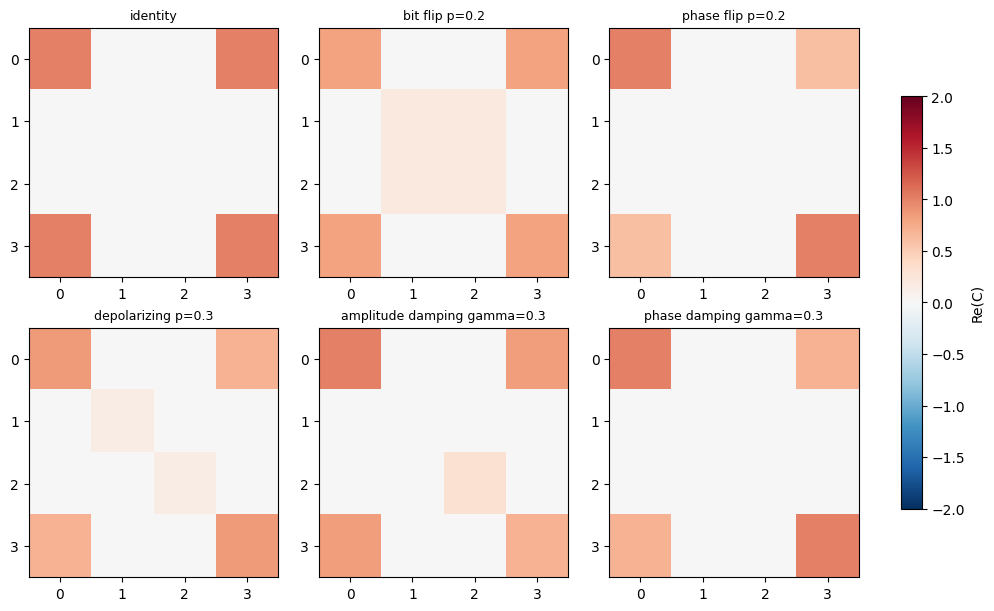
\includegraphics[width=0.94\textwidth]{fig_01_theory_01_cell6.png}
\caption{대표적인 qubit channel들의 Choi 행렬 실수부 비교. Identity channel은 rank가 1인 순수한 구조를 보이고, depolarizing channel은 대각 성분이 더 균일해지며, amplitude damping channel은 대칭적인 수축만이 아니라 특정 방향으로의 relaxation 구조가 나타난다. 이 그림은 채널의 물리적 성질이 Choi 행렬의 패턴에 직접 반영된다는 점을 보여준다.}
\label{fig:theory-choi-examples}
\end{figure}

그림 \ref{fig:theory-choi-examples}에서 가장 먼저 볼 부분은 identity channel과 잡음 채널의 차이이다. Identity channel의 Choi 행렬은 이상적인 maximally entangled 구조를 가지므로 특정 위치에 큰 coherence가 남아 있다. 반면 depolarizing channel에서는 상태가 균일한 혼합상태 쪽으로 밀리기 때문에 Choi 행렬의 뚜렷한 구조가 약해진다. 이는 Bloch sphere가 모든 방향으로 줄어드는 현상과 같은 내용이다.

Amplitude damping channel은 depolarizing channel과 다르게 단순한 균일 수축으로 설명되지 않는다. 이 채널은 excited state가 ground state로 내려가는 relaxation을 나타내므로, maximally mixed state도 그대로 보존하지 않는다. 따라서 TP 조건은 만족하지만 unital 조건은 만족하지 않는다. 이 결과는 TP와 unitality가 서로 다른 조건이라는 점을 잘 보여준다. TP는 전체 확률이 보존된다는 뜻이고, unitality는 항등연산자 또는 maximally mixed state가 보존된다는 뜻이다. 이렇게 그림에서 보이는 차이가 실제 계산에서도 같은 결론으로 이어지는지 확인하기 위해, 다음으로 CP/TP 판정과 표현 변환 오차를 수치적으로 비교하였다.

\subsection{수치 검증 결과}

표 \ref{tab:theory-results}는 이론 파트에서 확인한 대표적인 수치 결과이다. 변환 오차가 $10^{-16}$ 수준으로 나온 것은 double precision 계산에서 기대되는 round-off error와 같은 크기이다. 따라서 구현된 변환식이 서로 일관되게 작동한다고 볼 수 있다.

\begin{table}[H]
\centering
\small
\begin{tabularx}{\textwidth}{p{0.25\textwidth}p{0.31\textwidth}X}
\toprule
항목 & 관측값 & 해석 \\
\midrule
Identity channel & Choi rank $=1$ & 하나의 Kraus operator로 충분하므로 잡음 branch가 없다. \\
Depolarizing $p=0.3$ & min eigenvalue $=0.15$, TP=True, unital=True & 모든 Choi 고유값이 음수가 아니므로 CP이며, maximally mixed state를 보존한다. \\
Amplitude damping $\gamma=0.3$ & TP=True, unital=False, rank $=2$ & 확률은 보존하지만 Bloch sphere 중심이 이동하므로 unital하지 않다. \\
Random channel round-trip & error $\approx2.56\times10^{-16}$ & Choi에서 Kraus로 복원해도 원래 채널 작용과 machine precision 수준에서 일치한다. \\
Composition check & error $\approx2.48\times10^{-16}$ & natural form의 행렬곱이 channel composition과 일치한다. \\
\bottomrule
\end{tabularx}
\caption{이론 파트의 주요 수치 검증 결과}
\label{tab:theory-results}
\end{table}

특히 perturbed identity Choi 행렬이 CP=False로 판정된 예시는 중요하다. 행렬이 Hermitian이고 trace 조건을 거의 만족하더라도, 아주 작은 음의 고유값이 존재하면 완전양성성이 깨진다. 이는 tomography에서 raw reconstruction을 그대로 믿으면 안 되는 이유와 연결된다. 실제 실험에서는 shot noise 때문에 선형 역산 결과가 물리적으로 불가능한 Choi 행렬을 만들 수 있으며, 이 경우에는 CPTP projection이 필요하다.

\section{Process Tomography와 Choi 행렬 재구성}

\subsection{Tomography가 필요한 이유}

이론적으로 정의한 채널의 Choi 행렬은 코드로 바로 계산할 수 있다. 그러나 실제 장치에서 어떤 채널이 작용했는지는 직접 알 수 없다. 예를 들어 $X$ gate를 실행했다고 해도 실제로는 이상적인 $X$ 뒤에 amplitude damping, depolarizing noise, coherent error가 섞여 있을 수 있다. 따라서 여러 입력 상태를 넣고 출력 상태를 측정하여, 장치가 실제로 구현한 process를 재구성해야 한다. 이 절차가 process tomography이다.

Agent-2에서는 IBM hardware 실행을 염두에 둔 구조를 만들되, 보고서의 재현성을 위해 offline simulated data를 사용하였다. 이 선택은 실제 하드웨어 결과를 주장하기 위한 것이 아니라, tomography pipeline이 물리적으로 일관된 방식으로 작동하는지 확인하기 위한 것이다. 하드웨어 결과는 backend calibration, queue 상태, shot count에 따라 바뀔 수 있으므로, 고정된 fixture로 먼저 계산 흐름을 검증하는 것이 적절하다.

Offline simulation에서 기준이 되는 gate는 Qiskit \texttt{QuantumCircuit}으로 정의하였다. 그림 \ref{fig:qpt-target-circuits}의 $X$, $H$, CNOT 회로는 ideal Choi 행렬을 만들 때 사용하는 target circuit이다. 이후의 simulated noisy process는 이 ideal circuit 자체를 바꾸는 것이 아니라, target gate 뒤에 amplitude damping 또는 depolarizing channel을 붙인 stand-in channel로 구성하였다. 따라서 회로도는 tomography가 어떤 gate process를 기준으로 비교하는지를 보여 주고, 뒤의 Choi heatmap과 fidelity 표는 그 기준 process에 잡음이 섞이면 재구성 결과가 어떻게 달라지는지를 보여 준다.

\begin{figure}[H]
\centering
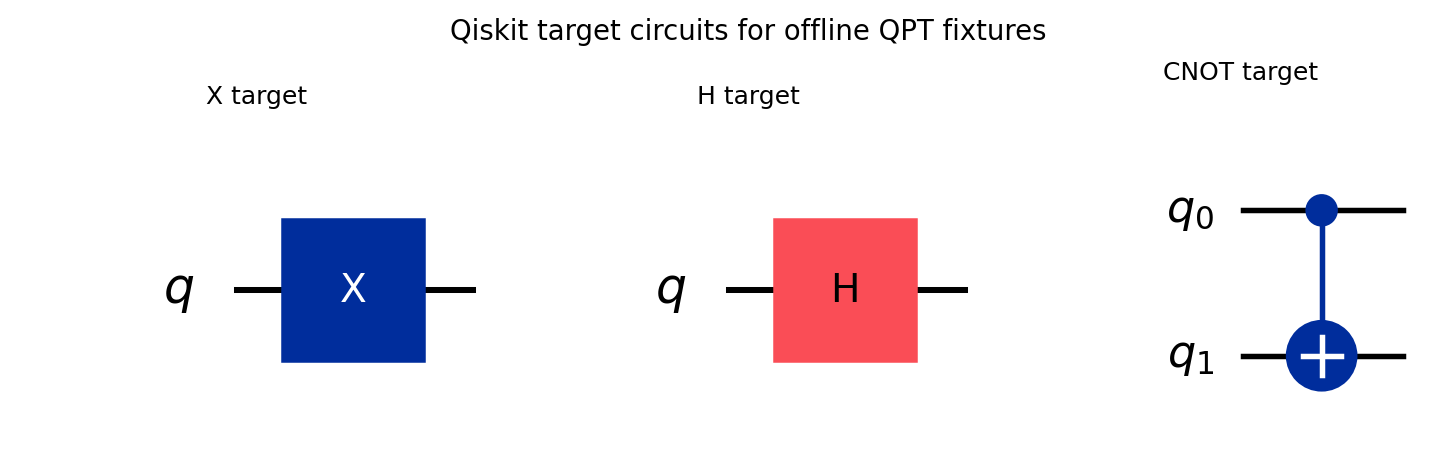
\includegraphics[width=0.92\textwidth]{fig_02_ibm_experiment_00_qiskit_circuits.png}
\caption{Offline QPT fixture에서 사용하는 Qiskit target circuits. $X$와 $H$는 one-qubit gate이고, CNOT은 control qubit $q_0$와 target qubit $q_1$에 작용하는 two-qubit gate이다. Noise model은 회로 안에 추가 gate로 그리지 않고, 이 target gate 뒤에 작용하는 Choi-level channel로 적용하였다.}
\label{fig:qpt-target-circuits}
\end{figure}

\subsection{이상적인 Choi 행렬과 재구성된 Choi 행렬}

Tomography 결과를 해석할 때 가장 먼저 확인해야 할 것은 재구성된 Choi 행렬이 이상적인 Choi 행렬의 큰 구조를 유지하는지이다. 큰 구조가 완전히 사라졌다면 게이트가 원하는 작용과 전혀 다른 process를 만든 것이고, 큰 구조는 유지되지만 작은 성분이 달라졌다면 이상적인 작용 위에 잡음이 섞인 것으로 해석할 수 있다. 이 구분을 위해 먼저 $X$ gate의 ideal Choi와 reconstructed Choi를 나란히 비교하였다.

\begin{figure}[H]
\centering
\begin{subfigure}{0.48\textwidth}
\centering
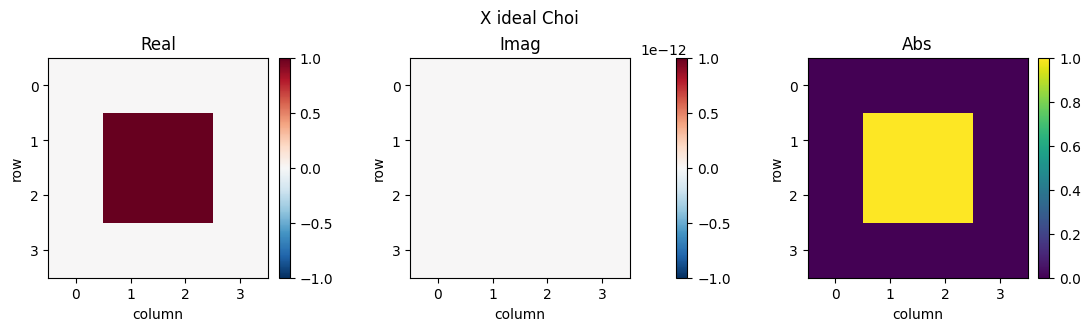
\includegraphics[width=\textwidth]{fig_02_ibm_experiment_01_cell20.png}
\caption{$X$ ideal Choi}
\end{subfigure}
\hfill
\begin{subfigure}{0.48\textwidth}
\centering
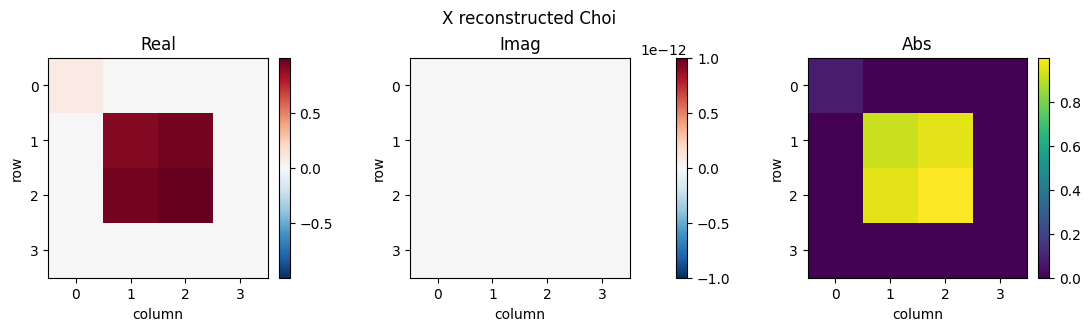
\includegraphics[width=\textwidth]{fig_02_ibm_experiment_02_cell20.png}
\caption{$X$ reconstructed Choi}
\end{subfigure}
\caption{$X$ gate의 이상적인 Choi 행렬과 재구성된 Choi 행렬 비교. 두 그림의 큰 구조는 비슷하지만 재구성된 행렬에서는 ideal pattern에서 벗어난 작은 성분들이 나타난다. 이는 gate가 완전히 틀렸다는 뜻이 아니라, 이상적인 unitary 과정에 잡음 성분이 섞였다는 뜻으로 해석된다.}
\label{fig:qpt-x-choi}
\end{figure}

그림 \ref{fig:qpt-x-choi}에서 reconstructed Choi가 ideal Choi와 완전히 같지 않은 것은 자연스러운 결과이다. 만약 두 행렬이 완전히 같다면 process fidelity는 1에 가까워지고 diamond distance는 0에 가까워야 한다. 실제 결과에서는 $X$ gate의 process fidelity가 0.959583으로 비교적 높게 나왔지만, half-diamond distance는 0.080000으로 0이 아니었다. 따라서 평균적인 관점에서는 이상적인 $X$와 상당히 가깝지만, 최적의 입력 상태를 선택하면 구별 가능한 차이가 남아 있다고 볼 수 있다.

$X$ gate 하나만 보면 이러한 차이가 특정 게이트에만 나타나는지, 아니면 분석 대상 전체에서 반복되는 경향인지 알기 어렵다. 그래서 다음으로 $X$, $H$, CNOT 세 게이트를 같은 지표로 비교하였다. 이 비교는 one-qubit gate와 two-qubit gate에서 잡음의 크기가 어떻게 다르게 나타나는지를 보기 위한 것이다.

\begin{figure}[H]
\centering
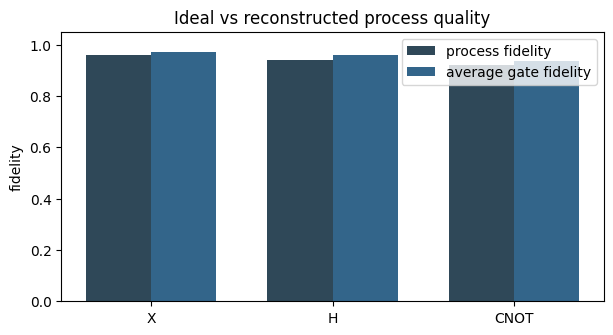
\includegraphics[width=0.74\textwidth]{fig_02_ibm_experiment_10_cell24.png}
\caption{$X$, $H$, CNOT에 대한 process fidelity와 average gate fidelity 비교. 모든 경우에서 fidelity가 1보다 작으므로 noise가 존재하며, CNOT의 fidelity가 상대적으로 낮게 나온다. 이는 two-qubit channel이 one-qubit channel보다 차원이 크고 noise branch가 많아지기 때문으로 생각된다.}
\label{fig:qpt-fidelity-bars}
\end{figure}

그림 \ref{fig:qpt-fidelity-bars}에서 CNOT의 process fidelity가 가장 낮게 나타났다. 이는 CNOT 자체가 두 qubit에 작용하므로 Choi 행렬의 차원이 커지고, global depolarizing noise가 붙으면 가능한 Pauli error branch의 수가 많아지기 때문이다. 따라서 동일한 noise strength처럼 보이더라도 two-qubit gate에서는 더 많은 방향으로 오차가 퍼질 수 있다. 이 결과를 실제 하드웨어 성능이라고 결론 내리기는 어렵지만, 분석 pipeline이 one-qubit와 two-qubit process를 같은 방식으로 비교할 수 있음을 보여준다.

다만 fidelity 막대그래프만으로는 잡음이 어떤 방향으로 작용했는지 알 수 없다. 예를 들어 fidelity가 비슷하게 낮아져도, 한 경우에는 모든 방향으로 균일하게 수축했을 수 있고 다른 경우에는 특정 축으로 상태가 이동했을 수 있다. 이 차이를 확인하기 위해 one-qubit channel에 대해서는 Bloch sphere 변형을 함께 보았다.

\begin{figure}[H]
\centering
\begin{subfigure}{0.47\textwidth}
\centering
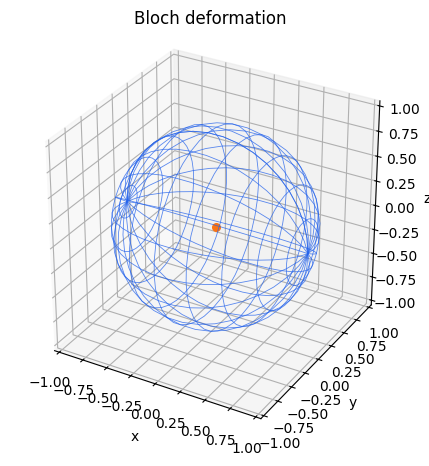
\includegraphics[width=0.82\textwidth]{fig_02_ibm_experiment_07_cell22.png}
\caption{$X$ reconstructed channel}
\end{subfigure}
\hfill
\begin{subfigure}{0.47\textwidth}
\centering
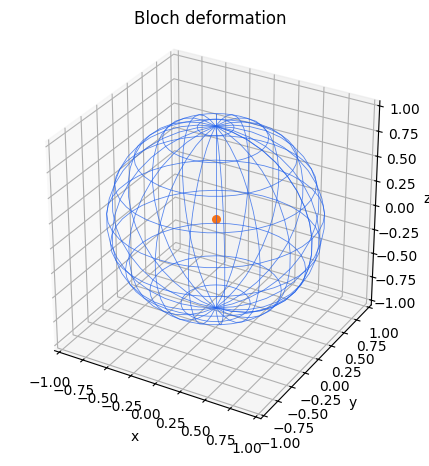
\includegraphics[width=0.82\textwidth]{fig_02_ibm_experiment_08_cell22.png}
\caption{$H$ reconstructed channel}
\end{subfigure}
\caption{재구성된 one-qubit channel의 Bloch sphere 변형. Depolarizing-like noise는 전체 구를 비교적 균일하게 줄이는 반면, amplitude-damping-like relaxation은 중심 이동을 동반한다. 따라서 Bloch sphere 그림은 fidelity 숫자만으로 보이지 않는 noise의 방향성을 보여준다.}
\label{fig:qpt-bloch}
\end{figure}

그림 \ref{fig:qpt-bloch}는 fidelity만으로는 설명하기 어려운 부분을 보완한다. Fidelity는 하나의 숫자로 process의 평균적인 유사도를 말해주지만, 잡음이 어느 방향으로 작용하는지는 직접 보여주지 않는다. 반면 Bloch sphere deformation을 보면 구가 균일하게 줄어드는지, 특정 방향으로 이동하는지, 특정 축이 더 많이 줄어드는지를 확인할 수 있다. $X$ gate에서 amplitude-damping-like relaxation이 진단된 것은 중심 이동과 관련이 있으며, $H$ gate에서 depolarizing-like shrinkage가 나타난 것은 방향성이 강한 이동보다 전체적인 수축이 두드러졌기 때문으로 해석된다.

이 진단은 그림만 보고 정성적으로 붙인 label이 아니라, 재구성된 Choi 행렬을 Pauli-transfer representation으로 바꾼 뒤 Bloch affine action을 계산하여 얻은 것이다. Ideal gate의 작용을 제거한 residual channel을
\[
r\mapsto Mr+t
\]
로 보았을 때, $t$의 norm이 크면 Bloch sphere 중심 이동이 있으므로 relaxation-like noise로 분류하고, $t$가 거의 0이면서 $M$의 singular value들이 거의 같은 비율로 작아지면 depolarizing-like shrinkage로 분류하였다. 표 \ref{tab:qpt-bloch-diagnostics}는 이 기준에 사용된 수치값을 정리한 것이다.

\begin{table}[H]
\centering
\small
\begin{tabularx}{\textwidth}{lcccX}
\toprule
Gate & $\|t\|_2$ & Singular-value spread & Mean shrinkage & 진단 근거 \\
\midrule
$X$ & 0.07999965 & 0.03916625 & 0.94611071 & 중심 이동 norm이 threshold 0.05보다 크므로 amplitude-damping-like relaxation으로 분류된다. \\
$H$ & $1.999\times10^{-15}$ & $1.999\times10^{-12}$ & 0.92000000 & 중심 이동과 축별 spread가 거의 0이고 전체 수축이 뚜렷하므로 depolarizing-like isotropic shrinkage로 분류된다. \\
\bottomrule
\end{tabularx}
\caption{One-qubit reconstructed channel의 Bloch affine 진단 수치. $\|t\|_2$는 Bloch sphere 중심 이동의 크기이고, singular-value spread는 세 Bloch 축의 수축 정도가 서로 얼마나 다른지를 나타낸다.}
\label{tab:qpt-bloch-diagnostics}
\end{table}

따라서 tomography 결과는 Choi heatmap, fidelity, Bloch sphere를 함께 보아야 안정적으로 해석된다. Heatmap은 ideal process와 reconstructed process의 구조적 차이를 보여주고, fidelity는 그 차이를 숫자로 요약하며, Bloch sphere는 그 차이가 어떤 물리적 잡음 모양으로 나타나는지 보여준다. 이 세 관찰을 정리한 값이 표 \ref{tab:qpt-results}이다.

\begin{table}[H]
\centering
\small
\begin{tabularx}{\textwidth}{lcccX}
\toprule
Gate & $F_{\mathrm{pro}}$ & $F_{\mathrm{avg}}$ & Half-diamond distance & 진단 \\
\midrule
$X$ & 0.959583 & 0.973055 & 0.080000 & amplitude-damping-like relaxation \\
$H$ & 0.940000 & 0.960000 & 0.060000 & depolarizing-like isotropic shrinkage \\
CNOT & 0.920000 & 0.936000 & 0.080000 & stochastic global depolarizing-like noise \\
\bottomrule
\end{tabularx}
\caption{Offline simulated QPT 결과}
\label{tab:qpt-results}
\end{table}

Linear inversion perturbation 예시에서는 minimum eigenvalue가 $-0.270000$으로 나와 CP 조건이 깨졌다. 이 값은 단순한 수치 오차라고 보기에는 너무 크다. 따라서 raw reconstruction은 물리적 채널로 받아들이기 어렵고, MLE 또는 CPTP projection을 통해 가장 가까운 물리적 Choi 행렬을 찾아야 한다. 이 과정은 실험 결과를 예쁘게 만들기 위한 후처리가 아니라, density matrix와 channel이 반드시 만족해야 하는 물리 법칙을 회복하는 과정이다.

\section{Channel Discrimination과 SDP}

\subsection{Diamond norm을 계산하는 이유}

Fidelity는 두 채널이 평균적으로 얼마나 비슷한지 알려주지만, 두 채널을 실제 실험에서 얼마나 잘 구별할 수 있는지는 별개의 문제이다. 동일한 prior probability로 두 채널 $\E_0$, $\E_1$ 중 하나가 주어졌다고 할 때, 최적 성공확률은
\[
p_{\mathrm{succ}}^{\max}
=\frac12+\frac14\|\E_0-\E_1\|_\diamond
\]
로 주어진다. 여기서 diamond norm은 reference system과의 entanglement까지 허용했을 때의 최적 구별 능력을 나타낸다.

이 점이 중요한 이유는 product input만 사용할 때와 entangled reference를 함께 사용할 때의 성능이 달라질 수 있기 때문이다. Choi 행렬은 SDP의 입력으로 사용되며, SDP는 가능한 모든 입력 전략 중 최적인 것을 찾는다. 따라서 channel discrimination 파트는 Choi 표현이 단순한 행렬 표현을 넘어서 실험적으로 의미 있는 성공확률과 연결된다는 것을 보여준다.

먼저 가장 해석하기 쉬운 경우로 depolarizing channel의 parameter가 바뀔 때 성공확률이 어떻게 변하는지 보았다. 이 예시는 두 채널의 차이가 커질수록 구별이 쉬워진다는 기본적인 직관을 확인하는 역할을 한다. 이 기본 경향이 확인되어야, 뒤에서 entanglement나 반복 사용이 주는 추가적인 이점을 더 분명하게 해석할 수 있다.

\begin{figure}[H]
\centering
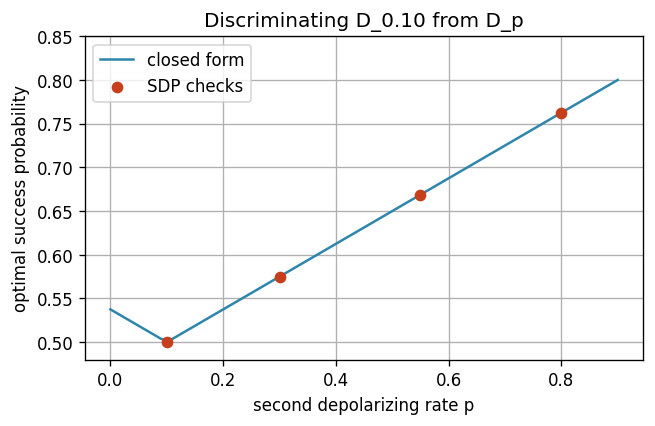
\includegraphics[width=0.72\textwidth]{fig_03_sdp_discrimination_01_cell9.png}
\caption{Depolarizing channel parameter가 달라질 때의 discrimination success probability. 기준 parameter와 비교 대상 parameter가 가까울수록 성공확률은 0.5에 가까워지고, 멀어질수록 성공확률이 증가한다. 이는 두 채널의 작용이 비슷하면 어떤 측정을 하더라도 구별하기 어렵다는 직관과 일치한다.}
\label{fig:sdp-depolarizing}
\end{figure}

그림 \ref{fig:sdp-depolarizing}에서 성공확률이 0.5 근처라는 것은 random guess와 큰 차이가 없다는 뜻이다. 기준 채널과 비교 채널의 depolarizing strength가 거의 같으면 출력 상태의 차이가 작아지므로 구별이 어려워진다. 반대로 parameter 차이가 커질수록 출력 상태들이 더 많이 달라지고, 이에 따라 최적 측정의 성공확률도 증가한다.

이제 문제는 단순히 parameter 차이가 클 때 성공확률이 올라간다는 데서 끝나지 않는다. 같은 두 채널을 구별하더라도 어떤 입력 전략을 쓰는지에 따라 성능이 달라질 수 있다. 특히 diamond norm은 reference system과의 entanglement까지 허용하므로, product input만 쓰는 경우와 ancilla-assisted input을 쓰는 경우를 비교해야 한다.

\begin{figure}[H]
\centering
\begin{subfigure}{0.48\textwidth}
\centering
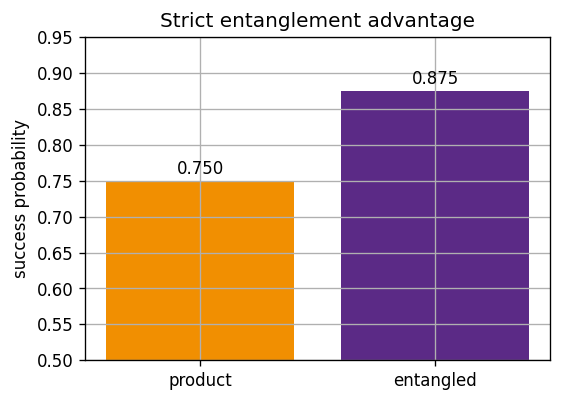
\includegraphics[width=\textwidth]{fig_03_sdp_discrimination_04_cell18.png}
\caption{Product input과 entangled input 비교}
\end{subfigure}
\hfill
\begin{subfigure}{0.48\textwidth}
\centering
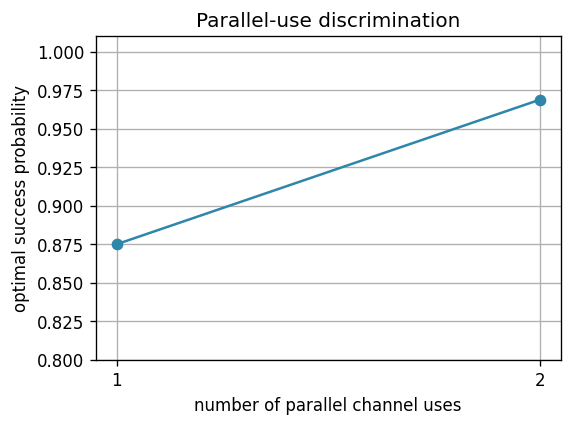
\includegraphics[width=\textwidth]{fig_03_sdp_discrimination_05_cell21.png}
\caption{Parallel channel use에 따른 성공확률}
\end{subfigure}
\caption{Channel discrimination에서 entanglement와 반복 사용이 주는 이점. Product input의 성공확률은 0.750000이었지만, ancilla-assisted input에서는 0.875000으로 증가하였다. 또한 2-shot parallel strategy에서는 0.968750까지 증가하였다.}
\label{fig:sdp-advantage}
\end{figure}

그림 \ref{fig:sdp-advantage}에서 product input과 entangled input 사이의 차이는 단순한 계산상 차이가 아니라 operational advantage이다. Product input만 사용하면 채널이 system에 남긴 차이만 볼 수 있다. 하지만 reference system과 entanglement를 만들고 채널이 system 쪽에만 작용하도록 하면, 채널의 작용이 joint state의 correlation에도 흔적을 남긴다. 이 추가 정보 때문에 성공확률이 증가한다.

2-shot 결과가 0.968750까지 올라간 것도 자연스럽다. 같은 channel을 여러 번 사용할 수 있으면 한 번의 출력보다 더 많은 정보를 얻을 수 있고, 두 채널의 차이가 누적된다. 다만 이 방법은 channel use 횟수가 증가할수록 Hilbert space 차원이 빠르게 커진다. 따라서 작은 예제에서는 효과가 명확하지만, 큰 system에서는 SDP의 계산 비용이 곧 한계가 된다. 이러한 관찰을 수치로 정리하면 표 \ref{tab:sdp-results}와 같다. 표는 Choi 행렬을 사용한 SDP가 단순한 유사도 계산이 아니라, 실제 구별 전략의 성공확률을 비교하는 도구임을 보여준다.

\begin{table}[H]
\centering
\begin{tabular}{lcc}
\toprule
전략 & 성공확률 & 해석 \\
\midrule
Bit-flip closed-form 검증 & 0.625000 & analytical diamond norm과 SDP 결과가 일치한다. \\
Product input & 0.750000 & reference 없이 가능한 최선의 성능이다. \\
Ancilla-assisted input & 0.875000 & entanglement가 구별 능력을 높인다. \\
2-shot parallel & 0.968750 & channel use가 늘어나며 차이가 누적된다. \\
\bottomrule
\end{tabular}
\caption{SDP 기반 channel discrimination의 주요 결과}
\label{tab:sdp-results}
\end{table}

\section{Non-Markovian Dynamics와 Quantum Combs}

\subsection{단일 시점 채널의 한계}

단일 Choi 행렬은 하나의 input-output 관계를 설명한다. 그러나 시간에 따른 과정에서 system이 environment와 여러 번 상호작용하고, 그 environment가 다음 시점에도 기억을 갖고 남아 있다면 단일 시점 채널만으로 전체 process를 설명하기 어렵다. 각 시점의 marginal channel은 모두 물리적인 CPTP channel처럼 보일 수 있지만, 그 사이에 시간 상관이 남아 있으면 전체 과정은 memoryless product로 분해되지 않는다.

이 경우 필요한 것이 quantum comb 또는 process tensor 관점이다. Quantum comb는 여러 time slot의 input-output 관계를 하나의 큰 Choi-like operator로 나타낸다. 따라서 단일 채널에서는 보이지 않던 시간 상관, memory residue, factorization failure를 확인할 수 있다.

먼저 memory effect가 실제 시간 신호에서 어떻게 보이는지 확인하기 위해 trace distance의 시간 변화를 보았다. Trace distance는 두 상태를 얼마나 잘 구별할 수 있는지를 나타내므로, 시간이 지날수록 줄어드는 것이 일반적인 잡음 과정의 모습이다. 만약 중간에 다시 증가한다면, 한때 environment로 빠져나갔던 정보가 system으로 되돌아왔다고 해석할 수 있다.

\begin{figure}[H]
\centering
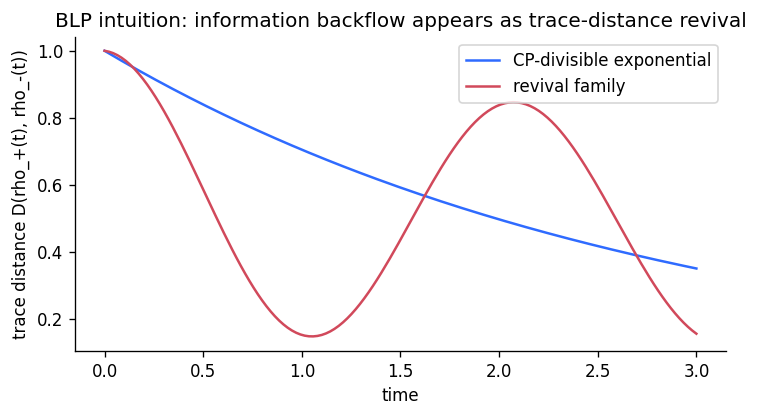
\includegraphics[width=0.76\textwidth]{fig_04_quantum_combs_01_cell7.png}
\caption{Markovian dephasing과 revival dephasing에서 trace distance의 시간 변화. Markovian dephasing에서는 trace distance가 단조 감소하지만, revival dephasing에서는 중간에 다시 증가하는 구간이 나타난다. 이 증가는 environment로 빠져나갔던 정보가 system으로 되돌아오는 현상으로 해석된다.}
\label{fig:comb-trace-distance}
\end{figure}

그림 \ref{fig:comb-trace-distance}에서 exponential dephasing의 trace distance는 계속 줄어든다. 이는 두 상태를 구별할 수 있는 정보가 시간이 지나며 줄어드는 상황이다. 반대로 revival dephasing에서는 trace distance가 다시 증가하는 구간이 존재한다. 이 증가는 단순한 노이즈 증가가 아니라, 이전에 environment로 흘러나갔던 정보가 system 쪽으로 일부 되돌아온 것으로 해석된다. 따라서 BLP witness가 양의 값을 갖는다.

그러나 trace distance 곡선만으로는 multi-time process 전체의 구조를 직접 볼 수 없다. 정보가 되돌아오는 현상을 더 구조적으로 확인하려면, 각 time slot을 따로 보는 대신 전체 two-use process를 하나의 comb로 놓고 memoryless product와 비교해야 한다.

\begin{figure}[H]
\centering
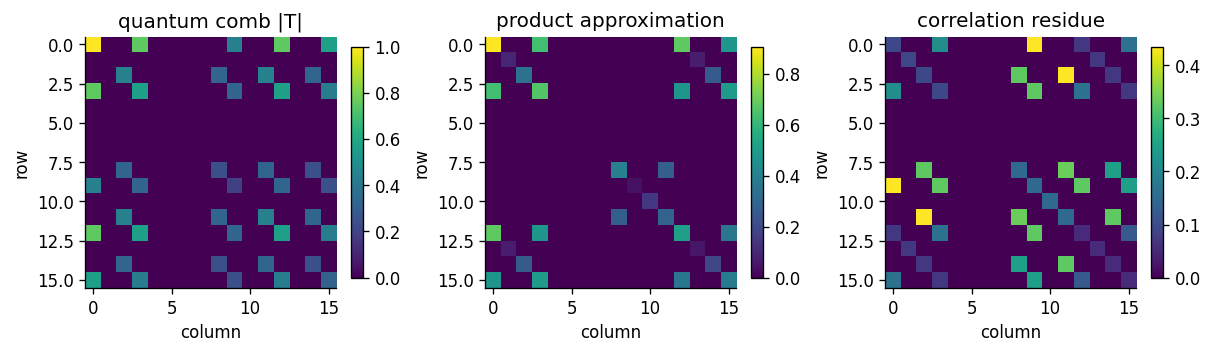
\includegraphics[width=0.92\textwidth]{fig_04_quantum_combs_02_cell10.png}
\caption{Two-use collision model에서 얻은 comb, memoryless product comb, 그리고 두 행렬의 차이. 두 marginal channel이 각각 물리적이더라도 전체 comb가 product form과 다르면 time slot 사이의 correlation이 남아 있다는 뜻이다.}
\label{fig:comb-correlation}
\end{figure}

그림 \ref{fig:comb-correlation}은 quantum comb 분석의 핵심을 보여준다. 왼쪽의 comb는 실제 collision model에서 얻은 전체 process이고, 가운데는 각 time slot의 marginal channel을 곱해서 만든 memoryless product approximation이다. 오른쪽의 차이가 0이 아니라는 것은 전체 process가 단순히 독립적인 두 channel의 연속으로 설명되지 않는다는 뜻이다.

수치적으로 comb matrix의 크기는 $(16,16)$이었고, minimum eigenvalue는 $-1.774\times10^{-16}$이었다. 이 값은 음수이긴 하지만 double precision round-off error 수준이므로 물리적으로는 0으로 보는 것이 타당하다. 또한 deterministic comb causality hierarchy도 True로 확인되었다. 따라서 constructed comb는 물리적 조건을 만족한다고 볼 수 있다. 반면 product marginal factorization은 False였고, relative comb correlation norm은 약 0.5307이었다. 이 값이 0이 아니라는 점이 memory effect의 핵심 증거이다.

여기서 주의할 점은 각 time slot의 marginal channel이 이상해 보여서 memory effect가 생기는 것이 아니라는 점이다. 오히려 marginal channel은 각각 정상적인 single-step channel처럼 보일 수 있다. 그래서 다음 그림에서는 marginal Choi 행렬만 따로 보았을 때와 전체 comb를 보았을 때의 차이를 확인하였다.

\begin{figure}[H]
\centering
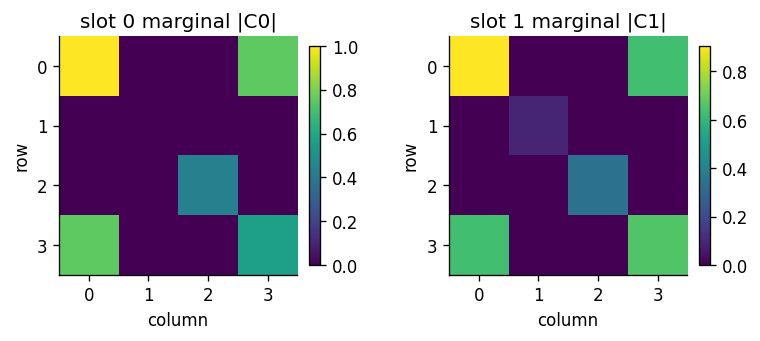
\includegraphics[width=0.72\textwidth]{fig_04_quantum_combs_03_cell13.png}
\caption{Two-use comb의 각 slot marginal Choi 행렬. 각 marginal만 보면 정상적인 single-step channel처럼 보이지만, marginal들의 곱만으로 전체 comb를 재구성할 수 없었다. 따라서 memory effect는 개별 시점의 채널이 아니라 시점 사이의 correlation에서 나타난다.}
\label{fig:comb-marginals}
\end{figure}

그림 \ref{fig:comb-marginals}는 왜 marginal channel만 보는 것이 부족한지 보여준다. 각 slot의 Choi 행렬은 그 자체로는 별다른 문제가 없어 보인다. 그러나 전체 comb와 product comb를 비교하면 차이가 남는다. 이는 실험에서 매 시점마다 정상적인 channel을 얻었다고 해서 전체 과정이 Markovian이라고 결론 내릴 수 없다는 점을 의미한다. 이 결론은 앞에서 본 trace distance revival과 같은 방향을 가리킨다. 따라서 마지막으로 BLP와 RHP-style witness 값을 함께 정리하여, 곡선 기반 진단과 comb 기반 진단이 서로 모순되지 않는지 확인하였다.

\begin{table}[H]
\centering
\begin{tabular}{lcc}
\toprule
Channel family & BLP grid estimate & RHP-style grid witness \\
\midrule
Exponential dephasing & 0.000000 & 0.000000 \\
Revival dephasing & 0.699240 & 0.896321 \\
\bottomrule
\end{tabular}
\caption{비마르코프성 witness 결과}
\label{tab:nonmarkov-results}
\end{table}

표 \ref{tab:nonmarkov-results}에서 exponential dephasing은 BLP와 RHP-style witness가 모두 0이었다. 이는 trace distance가 다시 증가하지 않고, intermediate map에서도 CP-divisibility violation이 관찰되지 않았다는 뜻이다. 반면 revival dephasing에서는 두 witness가 모두 양의 값을 가졌다. 따라서 두 방식 모두 memory effect를 같은 방향으로 진단했다고 볼 수 있다.

\section{Interactive Widget과 시각적 해석}

Interactive widget은 Choi 행렬의 조건을 시각적으로 확인하기 위해 만들어졌다. 수식으로는 $C_{\E}\succeq0$와 $\Tr_B(C_{\E})=I_A$가 간단하게 보이지만, 실제 channel action에서 이 조건들이 어떤 모양으로 나타나는지 바로 떠올리기는 쉽지 않다. Widget은 parameter를 움직일 때 Choi heatmap, eigenspectrum, Kraus display, Bloch sphere deformation, CP/TP indicator가 함께 변하도록 구성되었다.

앞의 절들에서는 Choi 행렬을 이론 검증, tomography, SDP, comb 분석에 각각 사용하였다. Widget은 이 계산들을 별도의 결과로 흩어 놓지 않고 한 화면에서 연결한다는 점에서 의미가 있다. 예를 들어 amplitude damping을 선택하면, Choi 행렬의 패턴과 고유값뿐 아니라 Bloch sphere가 어떤 방향으로 변형되는지도 동시에 확인할 수 있다.

\begin{figure}[H]
\centering
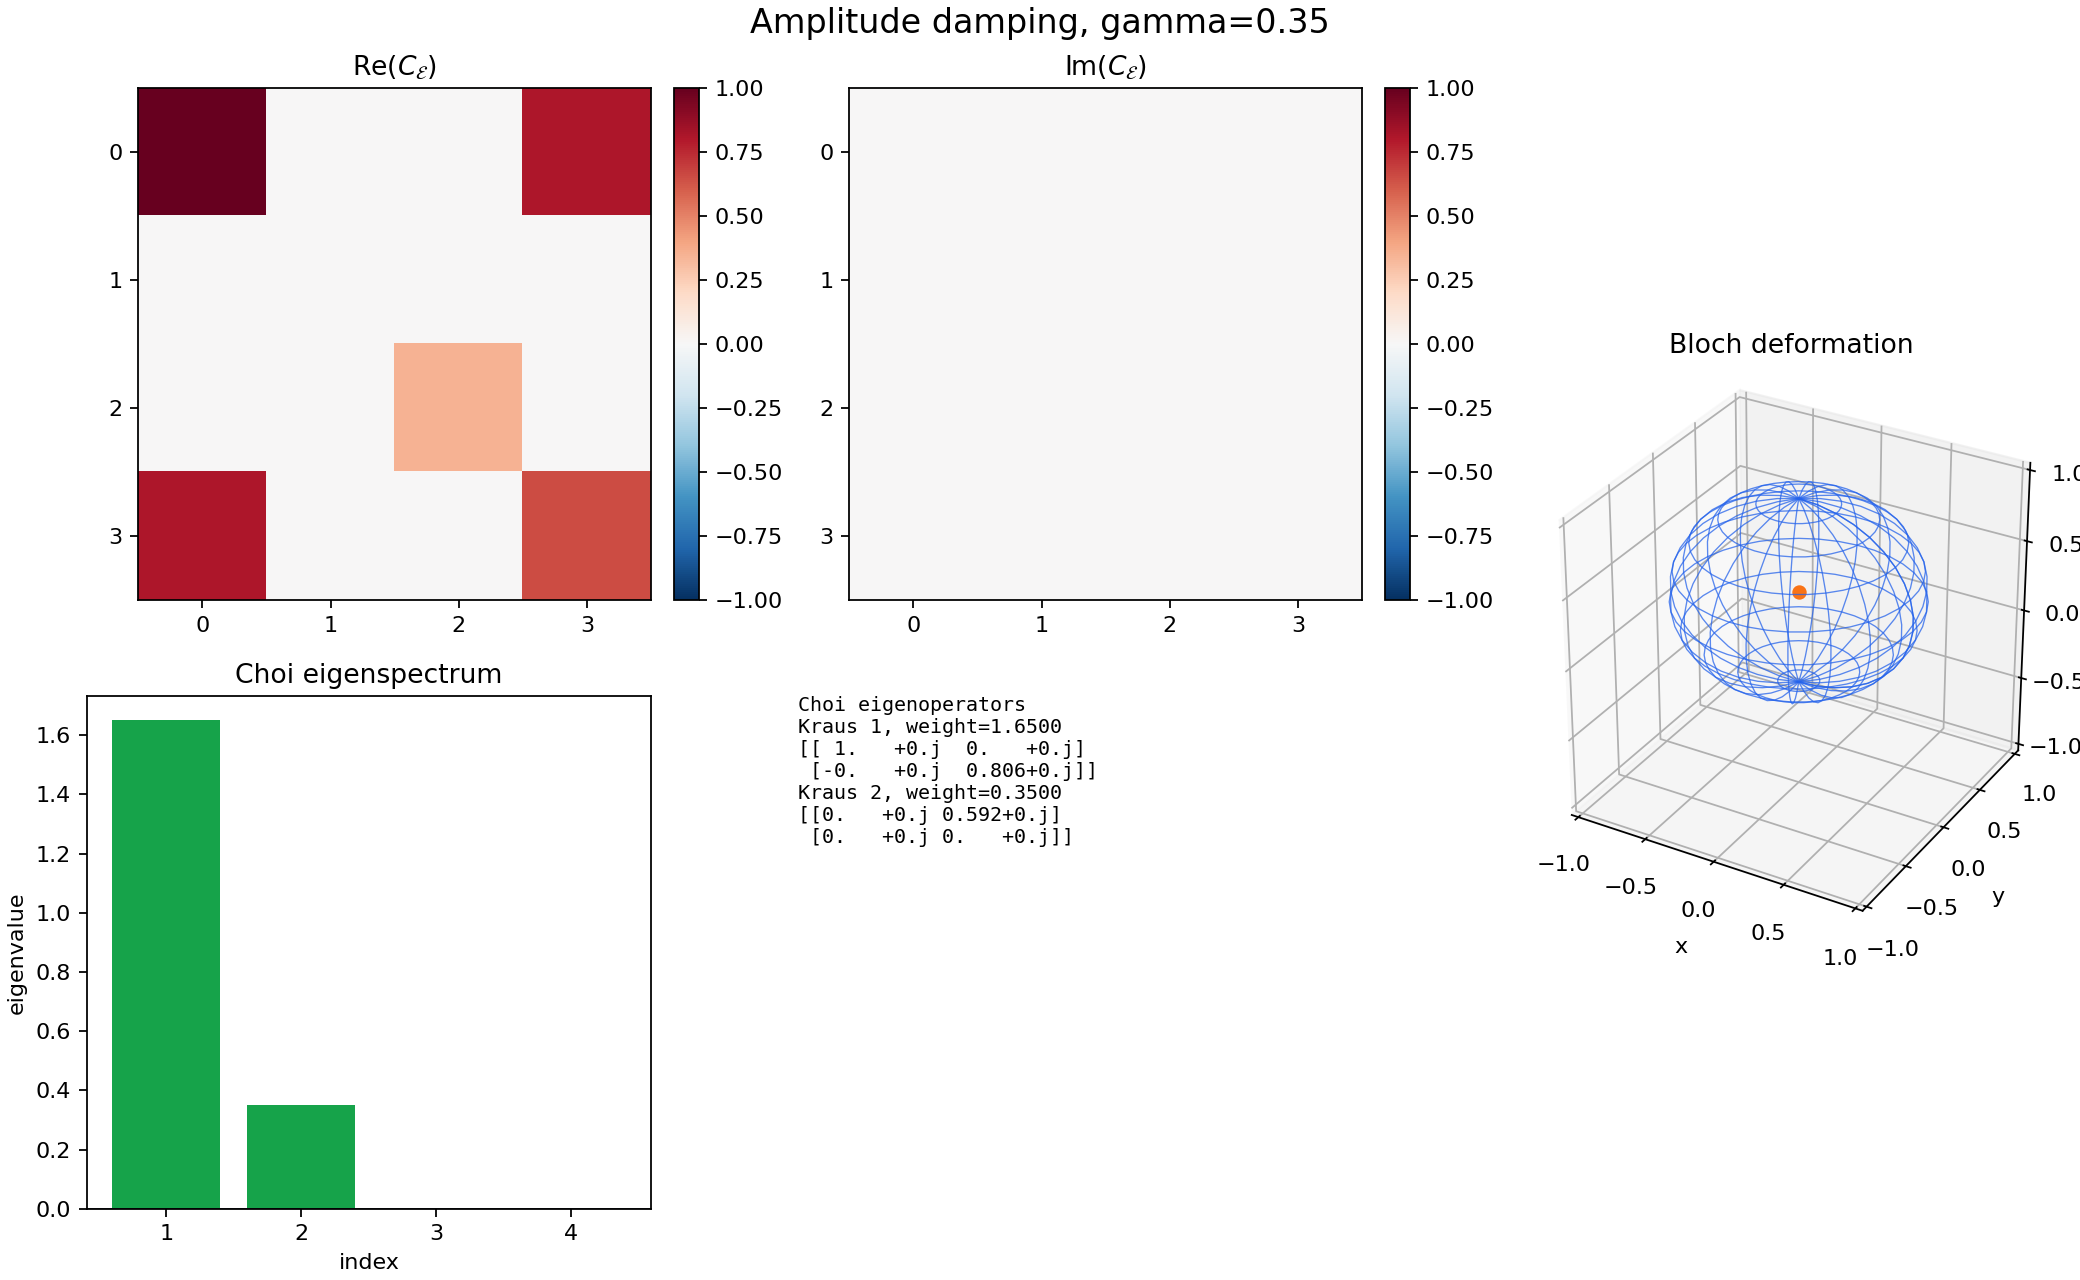
\includegraphics[width=0.94\textwidth]{fig_widget_dashboard.png}
\caption{Interactive widget의 amplitude damping 예시. 왼쪽에서는 Choi 행렬의 실수부, 허수부, 절댓값을 확인할 수 있고, 오른쪽에서는 Choi 고유값과 Bloch sphere 변형을 동시에 볼 수 있다. Amplitude damping에서는 Bloch sphere가 단순히 작아지는 것이 아니라 특정 방향으로 이동하므로, unital하지 않은 채널의 특징이 시각적으로 드러난다.}
\label{fig:widget-dashboard}
\end{figure}

그림 \ref{fig:widget-dashboard}에서 amplitude damping channel의 Bloch sphere는 중심을 유지한 채 균일하게 작아지는 형태가 아니다. 이는 depolarizing channel과 다른 점이다. Depolarizing channel은 모든 방향의 Bloch vector를 비슷하게 줄이므로 maximally mixed state가 중심에 남는다. 반면 amplitude damping은 excited state가 ground state로 내려가는 물리적 과정을 나타내므로 sphere의 중심 자체가 이동한다.

Widget에서 CP indicator가 Choi 고유값과 연결되어 있고, TP indicator가 partial trace와 연결되어 있다는 점도 중요하다. 사용자가 parameter를 변화시켜 CP 영역 밖으로 나가면 Choi eigenspectrum에서 음의 고유값이 나타난다. 이때 행렬이 겉보기에는 작은 변화만 겪은 것처럼 보여도, 물리적으로 가능한 채널은 아니게 된다. 따라서 widget은 단순한 시각화 도구라기보다 Agent-1의 이론 조건, Agent-2의 tomography 진단, Agent-3의 채널 차이 해석을 한 화면에서 연결하는 장치라고 볼 수 있다. 이 점 때문에 widget 절은 별도의 부록적 결과가 아니라, 프로젝트 전체를 다시 묶어 주는 마지막 연결 고리로 해석된다.

\section{통합 해석과 한계}

본 프로젝트의 가장 중요한 통합점은 Choi 행렬이 공통 interface로 작동했다는 점이다. Agent-1에서는 Choi 행렬이 채널 표현 변환과 CP/TP 판정의 기준이 되었다. Agent-2에서는 실험 또는 simulated tomography 데이터가 Choi 행렬로 재구성되며, fidelity와 noise diagnosis의 출발점이 되었다. Agent-3에서는 두 Choi 행렬의 차이가 SDP의 입력이 되어 optimal discrimination probability로 이어졌다. Agent-4에서는 Choi 관점이 여러 time slot으로 확장되어 quantum comb가 되었고, Agent-5에서는 같은 조건들이 시각적 widget으로 표현되었다.

\begin{longtable}{p{0.18\textwidth}p{0.32\textwidth}p{0.38\textwidth}}
\toprule
파트 & Choi 행렬의 역할 & 결과 해석 \\
\midrule
이론 & 표현 변환과 CP/TP 판정 & 채널 formalism의 계산 기준을 세웠다. \\
Tomography & 재구성된 process의 표현 & fidelity와 noise diagnosis를 가능하게 했다. \\
SDP & channel difference의 최적화 입력 & diamond norm으로 구별 가능성을 계산했다. \\
Combs & generalized Choi operator & time correlation과 memory residue를 나타냈다. \\
Widget & 시각적 대시보드 & 고유값, partial trace, Bloch deformation을 연결했다. \\
\bottomrule
\caption{Choi 표현의 통합적 역할}
\label{tab:integration}
\end{longtable}

결과를 종합하면, Choi 행렬은 단순한 수학적 변환이 아니라 실험과 계산을 이어주는 좌표계로 작동한다. 이론적으로는 물리성 조건을 판정하고, 실험적으로는 재구성된 process의 품질을 비교하며, 최적화에서는 operational success probability를 계산하고, 시간 과정에서는 memory structure를 드러낸다. 따라서 같은 행렬 표현을 유지한 덕분에 각 sub-topic의 결과가 서로 분리되지 않고 연결될 수 있었다.

한계도 분명하다. 대부분의 예제는 one-qubit 또는 small two-qubit system에 맞추어져 있다. Choi 행렬의 크기는 input과 output 차원의 곱에 대해 커지며, SDP variable은 그 행렬 전체를 다루어야 하므로 큰 system에서는 계산 비용이 빠르게 증가한다. Quantum comb 역시 time step 수가 늘어나면 차원이 지수적으로 증가한다. 따라서 이 방법들은 개념적으로 강력하지만, 큰 규모의 장치에 그대로 적용하려면 symmetry, tensor network, randomized protocol 같은 추가적인 압축 기법이 필요할 것이다.

또한 process tomography 결과는 offline simulated fixture를 기반으로 한다. 따라서 표에 제시된 fidelity와 diamond distance를 실제 IBM hardware 성능으로 해석하면 안 된다. 실제 hardware claim을 하려면 backend 이름, calibration 시각, shot count, job ID, raw count data, uncertainty estimate가 함께 제시되어야 한다. 본 보고서의 tomography 결과는 주로 분석 pipeline과 해석 방식의 검증으로 보는 것이 적절하다.

\section{결론}

본 프로젝트는 Choi 표현이 양자 채널 분석에서 왜 강력한 도구인지 여러 관점에서 확인하였다. 이론 파트에서는 Kraus, Choi, Stinespring, natural representation이 machine precision 수준에서 일관되게 변환됨을 보였다. Tomography 파트에서는 재구성된 Choi 행렬이 fidelity, diamond distance, Bloch sphere deformation을 통해 잡음의 크기와 방향성을 드러낸다는 것을 확인하였다. SDP 파트에서는 diamond norm이 channel discrimination 성공확률과 직접 연결되며, entangled reference와 parallel use가 실제로 성능을 향상시킬 수 있음을 보였다. Quantum comb 파트에서는 marginal channel이 정상적으로 보여도 전체 multi-time process에는 memory correlation이 남을 수 있음을 확인하였다. Widget 파트에서는 이러한 조건들을 한 화면에서 확인할 수 있도록 하여, 수식과 직관 사이의 간격을 줄였다.

전체적으로 보면 Choi 행렬은 채널의 물리성, 실험적 재구성, 최적 구별, 시간 상관, 시각화를 하나의 언어로 묶어준다. 특히 CP 조건이 고유값 조건으로, TP 조건이 partial trace 조건으로 바뀐다는 점은 계산과 해석 모두에서 큰 장점이다. 다만 큰 system으로 갈수록 Choi 행렬과 SDP의 크기가 빠르게 증가하므로, 향후에는 더 효율적인 표현과 근사 방법을 함께 고려해야 한다.

\section*{참고문헌}
\addcontentsline{toc}{section}{참고문헌}

\begin{itemize}
  \item M. A. Nielsen and I. L. Chuang, \textit{Quantum Computation and Quantum Information}. Cambridge University Press, 2010.
  \item M.-D. Choi, ``Completely positive linear maps on complex matrices,'' \textit{Linear Algebra and its Applications}, 1975.
  \item A. Jamio{\l}kowski, ``Linear transformations which preserve trace and positive semidefiniteness of operators,'' \textit{Reports on Mathematical Physics}, 1972.
  \item J. Watrous, \textit{The Theory of Quantum Information}. Cambridge University Press, 2018.
  \item G. Chiribella, G. M. D'Ariano, and P. Perinotti, ``Quantum circuit architecture,'' \textit{Physical Review Letters}, 2008.
  \item H.-P. Breuer, E.-M. Laine, and J. Piilo, ``Measure for the degree of non-Markovian behavior of quantum processes,'' \textit{Physical Review Letters}, 2009.
\end{itemize}

\end{document}
